\chapter{Ensemble Evaluation}
\label{chap:improvecompare}

The same evaluation methodology from Chapter~\ref{chap:experimentalsetting} used throughout the thesis is employed to compare the candidate methods of improving decision tree accuracy.
A total of ten algorithm variations are compared:
\begin{description}
\item[{\sc htnba}] Single Hoeffding tree with adaptive Naive Bayes prediction (Section~\ref{sec:leafexp}).\\
Used as the base method for bagging and boosting.
\item[{\sc bag3/5/10}] Oza and Russell's online bagging (Section~\ref{sec:baggingstream}).\\
Ensemble of three, five or ten {\sc htnba} trees.
\item[{\sc boost3/5/10}] Oza and Russell's online boosting (Section~\ref{sec:boostingstream}).\\
Ensemble of three, five or ten {\sc htnba} trees.
\item[{\sc hot3/5/10}] Hoeffding option tree (Section~\ref{sec:hot}).\\
Maximum of three, five or ten options per example.\\
Settings same as {\sc htnba} including adaptive Naive Bayes prediction.\\
Secondary split confidence $\delta'$ = 0.999
\end{description}
As previously, there are three memory-limited environments (100KB/sensor, 32MB/handheld, 400MB/server), 19 synthetic data sets, a limit of ten hours per training run, and testing via one million test examples. Training and testing speeds are listed as percentages of the full generation speeds unique to each data set as measured in Section~\ref{sec:genspeed}.

\section{Results}
\label{sec:ensexp}

\begin{table}
\caption{Final results averaged over all data sources comparing ensemble methods.}
\label{tab:ensavgs}
\centering
\begin{tabular}{|r|r|r|r|r|r|r|r|r|}
\hline
method	&
\rotatebox{90}{\parbox{9em}{accuracy\\(\%)}} &
\rotatebox{90}{\parbox{9em}{training examples\\(millions)}} &
\rotatebox{90}{\parbox{9em}{active leaves\\(hundreds)}} &
\rotatebox{90}{\parbox{9em}{inactive leaves\\(hundreds)}} &
\rotatebox{90}{\parbox{9em}{total nodes\\(hundreds)}} &
\rotatebox{90}{\parbox{9em}{(average) tree depth}}	&
\rotatebox{90}{\parbox{9em}{training speed (\%)}} &
\rotatebox{90}{\parbox{9em}{prediction speed (\%)}} \\
\hline
\multicolumn{9}{|c|}{100KB memory limit / sensor} \\
\hline
{\sc htnba} & 85.44 & 29 & 0 & 8.65 & 11.9 & 12 & 67 & 82 \\
{\sc bag3} & 85.82 & 6 & 0 & 7.66 & 10.4 & 7.8 & 54 & 67 \\
{\sc bag5} & 84.02 & 4 & 0 & 6.78 & 9.10 & 6.3 & 45 & 60 \\
{\sc bag10} & 78.34 & 2 & 0 & 5.49 & 7.40 & 4.6 & 37 & 52 \\
{\sc boost3} & 84.63 & 7 & 0 & 7.61 & 10.4 & 8.0 & 46 & 61 \\
{\sc boost5} & 83.67 & 4 & 0 & 6.82 & 9.30 & 6.5 & 37 & 53 \\
{\sc boost10} & 77.14 & 2 & 0 & 6.97 & 9.20 & 4.6 & 31 & 44 \\
{\sc hot3} & 86.34 & 15 & 0 & 8.83 & 11.5 & 12 & 54 & 68 \\
{\sc hot5} & 86.28 & 14 & 0 & 9.15 & 11.8 & 11 & 52 & 65 \\
{\sc hot10} & 85.90 & 14 & 0 & 9.60 & 12.1 & 11 & 52 & 63 \\
\hline
\multicolumn{9}{|c|}{32MB memory limit / handheld} \\
\hline
{\sc htnba} & 90.51 & 871 & 73.4 & 670 & 1106 & 24 & 14 & 65 \\
{\sc bag3} & 90.48 & 1025 & 34.1 & 1714 & 2539 & 20.0 & 16 & 50 \\
{\sc bag5} & 90.33 & 998 & 21.2 & 2064 & 3017 & 18.9 & 15 & 41 \\
{\sc bag10} & 90.34 & 825 & 13.0 & 2380 & 3458 & 17.6 & 16 & 30 \\
{\sc boost3} & 89.38 & 948 & 15.9 & 1994 & 3085 & 21.3 & 14 & 43 \\
{\sc boost5} & 89.60 & 1015 & 6.07 & 2240 & 3500 & 20.9 & 15 & 34 \\
{\sc boost10} & 89.33 & 814 & 1.81 & 2445 & 3774 & 19.4 & 14 & 23 \\
{\sc hot3} & 90.66 & 792 & 64.0 & 944 & 1481 & 23 & 13 & 55 \\
{\sc hot5} & 90.72 & 750 & 61.5 & 1005 & 1575 & 23 & 12 & 51 \\
{\sc hot10} & 90.70 & 691 & 59.6 & 1081 & 1687 & 22 & 11 & 49 \\
\hline
\multicolumn{9}{|c|}{400MB memory limit / server} \\
\hline
{\sc htnba} & 90.70 & 463 & 489 & 46.7 & 828 & 28 & 6 & 53 \\
{\sc bag3} & 90.73 & 332 & 917 & 252 & 1772 & 23.7 & 5 & 34 \\
{\sc bag5} & 90.68 & 257 & 998 & 672 & 2482 & 22.2 & 4 & 27 \\
{\sc bag10} & 90.79 & 173 & 1046 & 1476 & 3678 & 20.6 & 3 & 19 \\
{\sc boost3} & 89.77 & 156 & 985 & 869 & 2987 & 24.8 & 4 & 34 \\
{\sc boost5} & 90.01 & 109 & 1062 & 1492 & 4188 & 23.2 & 3 & 25 \\
{\sc boost10} & 89.93 & 79 & 1077 & 2994 & 6550 & 21.3 & 3 & 18 \\
{\sc hot3} & 90.85 & 377 & 580 & 73.9 & 1028 & 26 & 5 & 40 \\
{\sc hot5} & 90.94 & 344 & 608 & 86.1 & 1092 & 25 & 4 & 37 \\
{\sc hot10} & 90.96 & 292 & 609 & 133 & 1177 & 25 & 4 & 34 \\
\hline
\end{tabular}
\end{table}

Detailed per-data set results of the experiments are available in Appendix~\ref{sec:ensembleMethodTables}. To simplify comparison, averages across all data sets are compiled in Table~\ref{tab:ensavgs}. The general differences between memory environments follow the same trends seen in previous experiments---the most training examples are processed in 32MB of memory because once again the 100KB environment stops early once there is insufficient memory to continue growth, and the 400MB environment is slower due to deeper trees with many more active nodes to maintain.

The average accuracy figures clearly separate the methods. The {\sc hot} methods are the most accurate on average across all three environments, followed by the {\sc bag} methods. The {\sc boost} methods are the least accurate on average, in all cases worse than the average accuracy of a single {\sc htnba} tree.

It is interesting to study the accuracy trends when the number of trees, or equivalently the number of options, is increased in fixed memory limits. In the 100KB/sensor environment, higher ensemble sizes tend to be lower in accuracy, with ensembles of three trees being the most accurate size regardless of ensemble type. This trend is perhaps reflective of the size/accuracy tradeoff predicted in very limited memory. The 100KB is simply not enough to support accurate combinations of more than just a few trees.
In the 32MB/handheld environment the middle of the range size of five trees tends to be best, the most accurate size for boosted and option trees, and of the {\sc bag} methods only marginally worse than ten bagged trees. In the 400MB/server environment the generous memory allowance creates opportunities for the ten tree ensembles to do best, apart from boosting where {\sc boost5} is more accurate than {\sc boost10} on average.

In the 32MB and 400MB environments, the {\sc hot} methods tend to have smaller models than the other ensemble methods, with fewer tree nodes in total than either bagged or boosted trees. This is a positive result for the option tree representation. Boosted trees tend to have the most nodes on average.

\begin{table}
\caption{{\sc htnba} vs {\sc bag5} accuracy (\%).}
\label{tab:htnba_vs_bag5_acc}
\centering
\begin{tabular}{|r||r|r|r||r|r|r|}
\hline
method$\rightarrow$ & \multicolumn{3}{|c||}{{\sc htnba}} & \multicolumn{3}{|c|}{{\sc bag5}} \\
\hline
 & \multicolumn{3}{|c||}{memory limit} & \multicolumn{3}{|c|}{memory limit} \\
\hline
dataset & 100KB & 32MB & 400MB & 100KB & 32MB & 400MB \\
\hline
{\sc rts} & \textbf{96.92} & 99.99 & 99.99 & 84.84 & \textbf{100.00} & 99.99 \\
{\sc rtsn} & \textbf{74.91} & \textbf{78.49} & 78.44 & 69.82 & 78.48 & \textbf{78.49} \\
{\sc rtc} & \textbf{61.22} & \textbf{83.10} & \textbf{83.84} & 54.13 & 79.66 & 81.90 \\
{\sc rtcn} & \textbf{53.60} & \textbf{62.26} & \textbf{63.19} & 52.96 & 60.06 & 62.29 \\
{\sc rrbfs} & \textbf{88.43} & 93.60 & 93.84 & 87.68 & \textbf{93.93} & \textbf{94.29} \\
{\sc rrbfc} & \textbf{91.19} & 98.85 & 98.95 & 76.66 & \textbf{99.47} & \textbf{99.56} \\
{\sc wave21} & \textbf{81.23} & 84.80 & 85.66 & 81.01 & \textbf{85.19} & \textbf{86.14} \\
{\sc wave40} & \textbf{81.20} & 84.52 & 85.52 & 80.30 & \textbf{85.06} & \textbf{85.98} \\
{\sc led} & \textbf{73.96} & \textbf{74.02} & \textbf{73.98} & 73.35 & 73.98 & 73.97 \\
{\sc genF1} & 95.07 & 95.06 & \textbf{95.05} & 95.07 & \textbf{95.07} & 95.03 \\
{\sc genF2} & 78.30 & 94.05 & 94.05 & \textbf{92.18} & \textbf{94.11} & \textbf{94.09} \\
{\sc genF3} & 97.49 & \textbf{97.52} & \textbf{97.51} & \textbf{97.51} & 97.51 & 97.50 \\
{\sc genF4} & \textbf{93.86} & 94.68 & 94.65 & 91.61 & 94.68 & \textbf{94.66} \\
{\sc genF5} & 72.10 & 92.41 & 92.40 & \textbf{78.36} & \textbf{92.83} & \textbf{92.83} \\
{\sc genF6} & \textbf{92.09} & 93.31 & 93.29 & 90.64 & \textbf{93.34} & \textbf{93.32} \\
{\sc genF7} & \textbf{96.53} & 96.82 & 96.80 & 96.18 & \textbf{96.84} & \textbf{96.83} \\
{\sc genF8} & \textbf{99.41} & 99.42 & 99.42 & 99.40 & \textbf{99.43} & 99.42 \\
{\sc genF9} & \textbf{95.98} & 96.81 & 96.78 & 94.86 & \textbf{96.82} & \textbf{96.83} \\
{\sc genF10} & \textbf{99.89} & 99.89 & 99.89 & 99.88 & 99.89 & 99.89 \\
\hline
average & 85.44 & 90.51 & 90.70 & 84.02 & 90.33 & 90.68 \\
\hline
\end{tabular}
\end{table}

\begin{table}
\caption{{\sc htnba} vs {\sc boost5} accuracy (\%).}
\label{tab:htnba_vs_boost5_acc}
\centering
\begin{tabular}{|r||r|r|r||r|r|r|}
\hline
method$\rightarrow$ & \multicolumn{3}{|c||}{{\sc htnba}} & \multicolumn{3}{|c|}{{\sc boost5}} \\
\hline
 & \multicolumn{3}{|c||}{memory limit} & \multicolumn{3}{|c|}{memory limit} \\
\hline
dataset & 100KB & 32MB & 400MB & 100KB & 32MB & 400MB \\
\hline
{\sc rts} & \textbf{96.92} & 99.99 & \textbf{99.99} & 88.38 & 99.99 & 99.98 \\
{\sc rtsn} & \textbf{74.91} & \textbf{78.49} & \textbf{78.44} & 68.59 & 78.39 & 78.34 \\
{\sc rtc} & \textbf{61.22} & \textbf{83.10} & 83.84 & 59.23 & 82.39 & \textbf{84.24} \\
{\sc rtcn} & \textbf{53.60} & \textbf{62.26} & \textbf{63.19} & 53.55 & 59.27 & 60.12 \\
{\sc rrbfs} & \textbf{88.43} & \textbf{93.60} & \textbf{93.84} & 87.13 & 93.01 & 93.30 \\
{\sc rrbfc} & \textbf{91.19} & 98.85 & 98.95 & 79.87 & \textbf{99.19} & \textbf{99.30} \\
{\sc wave21} & \textbf{81.23} & \textbf{84.80} & \textbf{85.66} & 80.93 & 84.49 & 85.37 \\
{\sc wave40} & \textbf{81.20} & \textbf{84.52} & \textbf{85.52} & 80.48 & 84.32 & 85.06 \\
{\sc led} & \textbf{73.96} & \textbf{74.02} & \textbf{73.98} & 73.87 & 73.97 & 73.92 \\
{\sc genF1} & \textbf{95.07} & \textbf{95.06} & \textbf{95.05} & 93.72 & 90.93 & 93.23 \\
{\sc genF2} & 78.30 & \textbf{94.05} & \textbf{94.05} & \textbf{86.18} & 92.01 & 92.48 \\
{\sc genF3} & \textbf{97.49} & \textbf{97.52} & \textbf{97.51} & 96.40 & 95.47 & 96.41 \\
{\sc genF4} & \textbf{93.86} & \textbf{94.68} & \textbf{94.65} & 93.26 & 93.17 & 93.31 \\
{\sc genF5} & \textbf{72.10} & \textbf{92.41} & \textbf{92.40} & 68.72 & 91.80 & 91.66 \\
{\sc genF6} & \textbf{92.09} & \textbf{93.31} & \textbf{93.29} & 89.24 & 92.19 & 92.07 \\
{\sc genF7} & \textbf{96.53} & \textbf{96.82} & \textbf{96.80} & 95.93 & 96.14 & 96.02 \\
{\sc genF8} & \textbf{99.41} & \textbf{99.42} & \textbf{99.42} & 99.36 & 99.34 & 99.28 \\
{\sc genF9} & \textbf{95.98} & \textbf{96.81} & \textbf{96.78} & 94.93 & 96.43 & 96.21 \\
{\sc genF10} & \textbf{99.89} & \textbf{99.89} & \textbf{99.89} & 99.88 & 99.87 & 99.87 \\
\hline
average & 85.44 & 90.51 & 90.70 & 83.67 & 89.60 & 90.01 \\
\hline
\end{tabular}
\end{table}

\begin{table}
\caption{{\sc htnba} vs {\sc hot5} accuracy (\%).}
\label{tab:htnba_vs_hot5}
\centering
\begin{tabular}{|r||r|r|r||r|r|r|}
\hline
method$\rightarrow$ & \multicolumn{3}{|c||}{{\sc htnba}} & \multicolumn{3}{|c|}{{\sc hot5}} \\
\hline
 & \multicolumn{3}{|c||}{memory limit} & \multicolumn{3}{|c|}{memory limit} \\
\hline
dataset & 100KB & 32MB & 400MB & 100KB & 32MB & 400MB \\
\hline
{\sc rts} & \textbf{96.92} & 99.99 & 99.99 & 95.85 & 99.99 & 99.99 \\
{\sc rtsn} & \textbf{74.91} & \textbf{78.49} & \textbf{78.44} & 73.71 & 78.48 & 78.38 \\
{\sc rtc} & 61.22 & 83.10 & 83.84 & \textbf{64.79} & \textbf{84.22} & \textbf{84.92} \\
{\sc rtcn} & 53.60 & 62.26 & 63.19 & \textbf{54.64} & \textbf{63.88} & \textbf{65.61} \\
{\sc rrbfs} & \textbf{88.43} & 93.60 & 93.84 & 87.93 & \textbf{93.83} & \textbf{94.18} \\
{\sc rrbfc} & \textbf{91.19} & 98.85 & 98.95 & 78.63 & \textbf{99.20} & \textbf{99.22} \\
{\sc wave21} & 81.23 & 84.80 & 85.66 & 81.23 & \textbf{85.12} & \textbf{86.03} \\
{\sc wave40} & \textbf{81.20} & 84.52 & 85.52 & 81.14 & \textbf{84.95} & \textbf{85.86} \\
{\sc led} & \textbf{73.96} & \textbf{74.02} & \textbf{73.98} & 73.91 & 73.96 & 73.94 \\
{\sc genF1} & \textbf{95.07} & 95.06 & 95.05 & 95.06 & 95.06 & 95.05 \\
{\sc genF2} & 78.30 & 94.05 & 94.05 & \textbf{93.47} & \textbf{94.09} & \textbf{94.06} \\
{\sc genF3} & \textbf{97.49} & \textbf{97.52} & \textbf{97.51} & 97.48 & 97.51 & 97.50 \\
{\sc genF4} & \textbf{93.86} & \textbf{94.68} & \textbf{94.65} & 93.80 & 94.67 & 94.63 \\
{\sc genF5} & 72.10 & 92.41 & 92.40 & \textbf{84.25} & \textbf{92.71} & \textbf{92.80} \\
{\sc genF6} & \textbf{92.09} & 93.31 & \textbf{93.29} & 91.95 & \textbf{93.33} & 93.28 \\
{\sc genF7} & \textbf{96.53} & 96.82 & \textbf{96.80} & 96.38 & \textbf{96.83} & 96.79 \\
{\sc genF8} & \textbf{99.41} & 99.42 & 99.42 & 99.40 & 99.42 & 99.42 \\
{\sc genF9} & \textbf{95.98} & 96.81 & 96.78 & 95.77 & \textbf{96.82} & \textbf{96.79} \\
{\sc genF10} & \textbf{99.89} & 99.89 & 99.89 & 99.88 & 99.89 & 99.89 \\
\hline
average & 85.44 & 90.51 & 90.70 & 86.28 & 90.74 & 90.97 \\
\hline
\end{tabular}
\end{table}

\begin{table}
\caption{{\sc bag5} vs {\sc hot5} accuracy (\%).}
\label{tab:bag5_vs_hot5_acc}
\centering
\begin{tabular}{|r||r|r|r||r|r|r|}
\hline
method$\rightarrow$ & \multicolumn{3}{|c||}{{\sc bag5}} & \multicolumn{3}{|c|}{{\sc hot5}} \\
\hline
 & \multicolumn{3}{|c||}{memory limit} & \multicolumn{3}{|c|}{memory limit} \\
\hline
dataset & 100KB & 32MB & 400MB & 100KB & 32MB & 400MB \\
\hline
{\sc rts} & 84.84 & \textbf{100.00} & 99.99 & \textbf{95.85} & 99.99 & 99.99 \\
{\sc rtsn} & 69.82 & 78.48 & \textbf{78.49} & \textbf{73.71} & 78.48 & 78.38 \\
{\sc rtc} & 54.13 & 79.66 & 81.90 & \textbf{64.79} & \textbf{84.22} & \textbf{84.92} \\
{\sc rtcn} & 52.96 & 60.06 & 62.29 & \textbf{54.64} & \textbf{63.88} & \textbf{65.61} \\
{\sc rrbfs} & 87.68 & \textbf{93.93} & \textbf{94.29} & \textbf{87.93} & 93.83 & 94.18 \\
{\sc rrbfc} & 76.66 & \textbf{99.47} & \textbf{99.56} & \textbf{78.63} & 99.20 & 99.22 \\
{\sc wave21} & 81.01 & \textbf{85.19} & \textbf{86.14} & \textbf{81.23} & 85.12 & 86.03 \\
{\sc wave40} & 80.30 & \textbf{85.06} & \textbf{85.98} & \textbf{81.14} & 84.95 & 85.86 \\
{\sc led} & 73.35 & \textbf{73.98} & \textbf{73.97} & \textbf{73.91} & 73.96 & 73.94 \\
{\sc genF1} & \textbf{95.07} & \textbf{95.07} & 95.03 & 95.06 & 95.06 & \textbf{95.05} \\
{\sc genF2} & 92.18 & \textbf{94.11} & \textbf{94.09} & \textbf{93.47} & 94.09 & 94.06 \\
{\sc genF3} & \textbf{97.51} & 97.51 & 97.50 & 97.48 & 97.51 & 97.50 \\
{\sc genF4} & 91.61 & \textbf{94.68} & \textbf{94.66} & \textbf{93.80} & 94.67 & 94.63 \\
{\sc genF5} & 78.36 & \textbf{92.83} & \textbf{92.83} & \textbf{84.25} & 92.71 & 92.80 \\
{\sc genF6} & 90.64 & \textbf{93.34} & \textbf{93.32} & \textbf{91.95} & 93.33 & 93.28 \\
{\sc genF7} & 96.18 & \textbf{96.84} & \textbf{96.83} & \textbf{96.38} & 96.83 & 96.79 \\
{\sc genF8} & 99.40 & \textbf{99.43} & 99.42 & 99.40 & 99.42 & 99.42 \\
{\sc genF9} & 94.86 & 96.82 & \textbf{96.83} & \textbf{95.77} & 96.82 & 96.79 \\
{\sc genF10} & 99.88 & 99.89 & 99.89 & 99.88 & 99.89 & 99.89 \\
\hline
average & 84.02 & 90.33 & 90.68 & 86.28 & 90.74 & 90.97 \\
\hline
\end{tabular}
\end{table}

The average accuracy figures do not, however, convey the whole situation. Tables~\ref{tab:htnba_vs_bag5_acc}-\ref{tab:htnba_vs_hot5} give a detailed per-data set accuracy breakdown of a single {\sc htnba} tree against the mid-range ensembles (five trees/options). In Table~\ref{tab:htnba_vs_bag5_acc} the {\sc bag5} method does not compete well in 100KB of memory, but wins many times in the other environments. In Table~\ref{tab:htnba_vs_boost5_acc} the {\sc boost5} method struggles to show any gain over a single tree. In Table~\ref{tab:htnba_vs_hot5}, {\sc hot5} generally outperforms {\sc htnba}, but is not so convincing in the 100KB environment.

Table~\ref{tab:bag5_vs_hot5_acc} directly compares {\sc bag5} with {\sc hot5}. In 100KB of memory the option tree method is clearly superior. In the higher memory environments, {\sc hot5} is actually worse than {\sc bag5} in most cases. The main exception is the {\sc rtc}/{\sc rtcn} data sets where {\sc hot5} is ahead by such a margin that overall the average accuracy is higher (see Section~\ref{sec:boostdiscuss} for detailed analysis). This is a case where the average values are misleading. On the whole {\sc bag} and {\sc hot} are fairly similar with different strengths and weaknesses. One of the option trees clear strengths is memory efficiency---it is better than bagging in the most limited memory environment, and in general it uses fewer tree nodes while achieving similar accuracy.

\begin{figure}
\centering
\begin{tabular}{c@{}c}
\includegraphics[width=0.5\textwidth]{figures/rts-r1-400MB_ensacc} &
\includegraphics[width=0.5\textwidth]{figures/rts_opt_hist} \\
\includegraphics[width=0.5\textwidth]{figures/rtsn-r1-400MB_ensacc} &
\includegraphics[width=0.5\textwidth]{figures/rtsn_opt_hist} \\
\includegraphics[width=0.5\textwidth]{figures/rtc-r1-400MB_ensacc} &
\includegraphics[width=0.5\textwidth]{figures/rtc_opt_hist} \\
\includegraphics[width=0.5\textwidth]{figures/rtcn-r1-400MB_ensacc} &
\includegraphics[width=0.5\textwidth]{figures/rtcn_opt_hist} \\
\end{tabular}
\caption{Part 1 of learning curves for ensemble methods (left) and {\sc hot} option distribution (right) in 400MB memory limit.}
\label{fig:400MB_ens1}
\end{figure}

\begin{figure}
\centering
\begin{tabular}{c@{}c}
\includegraphics[width=0.5\textwidth]{figures/rrbfs-r1-400MB_ensacc} &
\includegraphics[width=0.5\textwidth]{figures/rrbfs_opt_hist} \\
\includegraphics[width=0.5\textwidth]{figures/rrbfc-r1-400MB_ensacc} &
\includegraphics[width=0.5\textwidth]{figures/rrbfc_opt_hist} \\
\includegraphics[width=0.5\textwidth]{figures/led-r1-400MB_ensacc} &
\includegraphics[width=0.5\textwidth]{figures/led_opt_hist} \\
\includegraphics[width=0.5\textwidth]{figures/wave21-r1-400MB_ensacc} &
\includegraphics[width=0.5\textwidth]{figures/wave21_opt_hist} \\
\end{tabular}
\caption{Part 2 of learning curves for ensemble methods (left) and {\sc hot} option distribution (right) in 400MB memory limit.}
\label{fig:400MB_ens2}
\end{figure}

\begin{figure}
\centering
\begin{tabular}{c@{}c}
\includegraphics[width=0.5\textwidth]{figures/wave40-r1-400MB_ensacc} &
\includegraphics[width=0.5\textwidth]{figures/wave40_opt_hist} \\
\includegraphics[width=0.5\textwidth]{figures/genF1-r1-400MB_ensacc} &
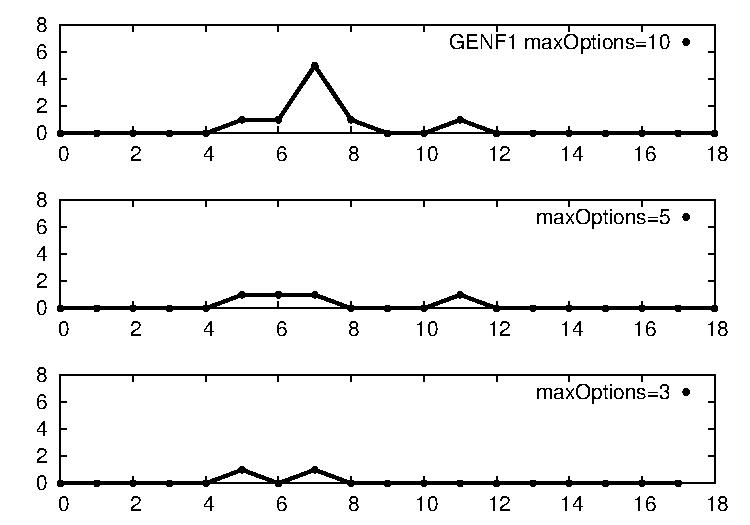
\includegraphics[width=0.5\textwidth]{figures/genF1_opt_hist} \\
\includegraphics[width=0.5\textwidth]{figures/genF2-r1-400MB_ensacc} &
\includegraphics[width=0.5\textwidth]{figures/genF2_opt_hist} \\
\includegraphics[width=0.5\textwidth]{figures/genF3-r1-400MB_ensacc} &
\includegraphics[width=0.5\textwidth]{figures/genF3_opt_hist} \\
\end{tabular}
\caption{Part 3 of learning curves for ensemble methods (left) and {\sc hot} option distribution (right) in 400MB memory limit.}
\label{fig:400MB_ens3}
\end{figure}

\begin{figure}
\centering
\begin{tabular}{c@{}c}
\includegraphics[width=0.5\textwidth]{figures/genF4-r1-400MB_ensacc} &
\includegraphics[width=0.5\textwidth]{figures/genF4_opt_hist} \\
\includegraphics[width=0.5\textwidth]{figures/genF5-r1-400MB_ensacc} &
\includegraphics[width=0.5\textwidth]{figures/genF5_opt_hist} \\
\includegraphics[width=0.5\textwidth]{figures/genF6-r1-400MB_ensacc} &
\includegraphics[width=0.5\textwidth]{figures/genF6_opt_hist} \\
\includegraphics[width=0.5\textwidth]{figures/genF7-r1-400MB_ensacc} &
\includegraphics[width=0.5\textwidth]{figures/genF7_opt_hist} \\
\end{tabular}
\caption{Part 4 of learning curves for ensemble methods (left) and {\sc hot} option distribution (right) in 400MB memory limit.}
\label{fig:400MB_ens4}
\end{figure}

\begin{figure}
\centering
\begin{tabular}{c@{}c}
\includegraphics[width=0.5\textwidth]{figures/genF8-r1-400MB_ensacc} &
\includegraphics[width=0.5\textwidth]{figures/genF8_opt_hist} \\
\includegraphics[width=0.5\textwidth]{figures/genF9-r1-400MB_ensacc} &
\includegraphics[width=0.5\textwidth]{figures/genF9_opt_hist} \\
\includegraphics[width=0.5\textwidth]{figures/genF10-r1-400MB_ensacc} &
\includegraphics[width=0.5\textwidth]{figures/genF10_opt_hist} \\
\end{tabular}
\caption{Part 5 of learning curves for ensemble methods (left) and {\sc hot} option distribution (right) in 400MB memory limit.}
\label{fig:400MB_ens5}
\end{figure}

Learning curves for all methods in 400MB are plotted on the left side of  Figures~\ref{fig:400MB_ens1}-\ref{fig:400MB_ens5}. The poor performance of boosting stands out most on the {\sc genF1}-{\sc genF10} data.

Alongside each learning curve plot are three plots displaying the distribution of extra options present in the final option trees. 
Plotted on the $y$-axis is the number of additional options introduced, and on the $x$-axis is the depth of the options.
The depth of zero represents the root of the tree, and the $x$-axis is scaled to accommodate the full depth of the tree. There are several cases where options were added at the root: {\sc rtc}, {\sc rtcn}, {\sc led}, {\sc wave21} and {\sc wave40}. In all other cases there were no additional options at the root. It is uncertain why this is the case, the maximum number of options are exceeded at the root before it is ready to introduce options. This may suggest that estimation at the root tends to be more reliable, or is perhaps due to the data sets having only a single attribute that splits well at the root.

Recall that Kohavi and Kunz~\cite{kohaviot} concluded that options nearer the root are more valuable. In general the option trees induced had their options present in the upper half of the tree. This is a side effect of the option limits and memory management. Options are allowed during early growth while the tree is shallow, but later when option limits and memory management prohibit introduction of further options the trees will continue to deepen, so it is not surprising that they tend to occur nearer the root of the tree.

\section{Discussion}
\label{sec:boostdiscuss}

Some of the results are puzzling---why does boosting do so poorly, and why does the option tree stand out against bagging on the {\sc rtcn} data source? To help gain greater understanding of differences between the methods, a bias/variance decomposition analysis is employed. The bias and variance components of the error were estimated on two selected data sets in 400MB of memory. This involved training the algorithms ten times on independent streams of ten million examples each, and testing on ten thousand held-out test examples. From this procedure the bias and variance were computed according to Kohavi and Wolpert~\cite{bvdecomp}. A smaller scale experiment was required to collect these results. Although not training each model as much as in the final experiments, repeating the procedure ten times makes it a time demanding process. Even though the results are based on smaller training sets they are still expected to expose meaningful differences between the methods.

\begin{figure}
\includegraphics{figures/rtcn_bias_variance}
\caption{Bias variance decomposition on {\sc rtcn}.}
\label{fig:rtcn_dvdecomp}
\end{figure}

\begin{figure}
\includegraphics{figures/wave21_bias_variance}
\caption{Bias variance decomposition on {\sc wave21}.}
\label{fig:wave21_dvdecomp}
\end{figure}

Figure~\ref{fig:rtcn_dvdecomp} shows the bias/variance decomposition estimates on the {\sc rtcn} data. On this particular data set in Section~\ref{sec:ensexp}, {\sc bag} did substantially worse than {\sc hot}. The bias of {\sc bag} and {\sc hot} is similar on this problem, close to the bias of a single tree, although the bias is relatively constant between the {\sc hot} sizes whereas it noticeably increases with the size of the {\sc bag} ensembles. The main difference lies in the estimated variance, which is reduced the most by {\sc hot} and also substantially reduces with larger {\sc bag} ensembles while not dropping quite as low. The combined effect of the components of error leads to an overall error in favour of {\sc hot}, which has the lowest error of all methods. {\sc bag} error falls closer to that of a single {\sc htnba} tree as more trees are combined, but as reflected in the final accuracy figures in Table~\ref{tab:htnba_vs_bag5_acc} it is not as accurate. On this particular data set, which is one of the most complex benchmark data sets tested, bagging has high variance with three trees and high bias with ten.
Either way it does not compete with the Hoeffding option tree which maintains a steady variance, and significantly lower bias that reduces slightly with additional options. Boosting manages to substantially reduce bias, much more than the other methods, but has consistently high variance, with overall error that is worse than the other methods.

Figure~\ref{fig:wave21_dvdecomp} displays the estimated bias/variance on the {\sc wave21} data. In experiments involving 32 and 400 megabytes of memory, {\sc bag} was generally superior to {\sc hot} on this problem (Table~\ref{tab:bag5_vs_hot5_acc}). Once again the bias of {\sc bag} increases with extra trees compared to the steady bias of {\sc hot}, both of which have more bias than a single tree. This time as the number of trees in the bag increases, {\sc bag} manages to reduce variance more than any other method, which results in the lowest errors overall when five or ten trees are combined. {\sc hot} is competitive but does not reduce the variance as significantly. Boosting excels at reducing bias, the lowest of the methods, but is less accurate again due to high variance.

Bias/variance decomposition analysis on these two data sets suggests the following trends: 

\begin{enumerate}
\item Both bagging and option trees are successful at reducing variance, which explains their ability to reduce error beyond a single tree. 
\item In terms of differences between bagging and option trees, adding trees to bagging tends to have stronger effects on bias and variance, whereas option trees are much more steady as additional options are introduced. On certain data sets, option trees can reduce the variance considerably more than bagging, but the majority of the time bagging has slightly outperformed option trees in this regard.
\item Boosting performs poorly due to high variance.
\end{enumerate}

The boosting result is disappointing considering that it offers so much promise in the batch setting. Transferring the generalization power of boosting from the batch setting to the data stream setting does not appear to be as trivial as one might think. The intuitive understanding of getting models to concentrate more on examples that are harder for previous models to classify gives the impression that it should be reproducible in the stream setting. After all, Breiman~\cite{arcing} set out to prove with arc-x4 that the ``magic'' of boosting does not lie in specific details.

The study of Brain and Webb~\cite{lowbiaslargeds} suggests that management of bias may be more important than managing variance on large data sets. Reducing bias is a difficult problem, boosting is most successful of
the tested methods but fails overall. This may partly be due to lack of space, and also since the hypothesis space is enlarged there is increased risk of choosing a poorer hypothesis.

Preliminary experimentation suggesting that boosting was not competing well with other methods motivated a search for an adaptation of boosting that is more successful. 
Attempted implementations included several direct {\em parallel} boosting adaptations of AdaBoost~\cite{adaboost}, including its confidence-rated version~\cite{boostimproved}. For example, following the half correct/half incorrect weighting observation exploited by Oza and Russell~\cite{ozabagboost} and inspired by Schapire's original hypothesis boosting algorithm~\cite{strength}, one attempt was to boost by filtering examples---subsequent models in sequence would get a correctly classified example followed by an incorrectly classified one, with any examples not conforming to the desired pattern being discarded. 
Other attempts included arc-x4~\cite{arcing}, MadaBoost~\cite{madaboost} and stream adaptations of the {\em alternating decision tree algorithm}~\cite{adtrees}. A few {\em block} boosting approaches were also investigated.
Successful application in the data stream setting was difficult to find despite Breiman's suggestion that the essential formula lies only in the adapting, resampling and combining process.

Oza and Russell's algorithm was chosen as the boosting representative because it performed among the best, it compliments the online bagging implementation and has literature to support it as a successful method. Unfortunately, when Oza and Russell demonstrate the ability of their method they do so without mention of fixed memory limits. Their experimental results~\cite{ozabagboost, ozaexp} using Utgoff's {\em ITI} decision tree algorithm~\cite{iti} as the base learner exhibit similar tendencies of online boosting competing poorly with online bagging. To improve the situation they try to bolster online boosting via ``priming'', which helps, but is not a solution explored by this thesis because it deviates from a purely stream-based solution. In their case they combine 100 trees, but note that in using ITI they are restricted to small data sets due to its poor scalability.

Deeper analysis of where the boosting attempts failed would often point towards problems with the example weighting process. Without a normalization step, it was observed that weights on particular examples in the stream grow uncontrollably, to the point where their magnitude exceeded the representational capacity of the machine. This problem is believed to represent a fundamental shortcoming of AdaBoost in streams. Domingo and Watanabe~\cite{madaboost} made a similar observation, which is why their MadaBoost algorithm limits the magnitude of example weights. Experimenting with simple solutions such as this removed the symptoms but also diluted the boosting procedure, and did not show signs of the spectacular generalization promised by boosting.

Why does this weighting problem occur on streamed data and not in the batch case? In the batch setting the weights are calculated over a known and fixed set of examples. In a stream, new examples are being continually introduced, potentially representing areas of the concept space that have not been encountered before. It is difficult to estimate sensible weights for these examples in relation to previous examples and previous weights.

AdaBoost was conceived as a boosting by {\em sampling} method, but what is really needed for successful data stream application is a boosting by {\em filtering} method. As reviewed in Section~\ref{sec:boostingbatch}, several researchers have attempted to supply such a method~\cite{madaboost, polyboost}, but the proposals so far have lacked the simplicity and elegance of AdaBoost. Intuitive and successful boosting in the data stream setting, that is on par with AdaBoost in the batch setting, remains an open problem.

The question of whether several models can provide benefit over a single model of the same size has been answered affirmatively, although the evidence suggests that plenty of memory is required to make ensembles worthwhile. In the highly restrictive 100KB environment a single tree is difficult to compete with, although the memory efficient option tree shows the most promise.

\section{Summary}

This experimental study looked at limited memory induction of decision tree ensembles from data streams.
Three main methods were explored---bagging and boosting, two ensemble methods that are very popular in batch learning, and the third a powerful tree representation known as option trees.
In empirical comparison bagging and option trees both showed ability to outperform a single tree, by significantly reducing the variance of individual trees, with varying strengths depending on the situation. Option trees were the most efficient in memory usage, showing the best ensemble performance in 100KB of memory, and showing significant improvement over bagging in a few 32MB/400MB cases. Overall bagging was able to outperform option trees in many other cases, a more consistent performer when sufficient memory is available. The general finding is that the more trees to be combined in an ensemble, the more memory needed to gain an advantage.
No successful implementation of boosting for data streams was found.
Boosting, or more specifically, AdaBoost, is perhaps the most powerful ensemble method known in batch learning. It is concluded that a truly successful and straightforward translation of AdaBoost to the data stream setting has yet to be discovered.

The change from a single {\sc htnba} tree to a Hoeffding option tree with
five options per example, {\sc hot5}, caused an increase in average accuracy
from 88.88\% to 89.31\%, which is a relative improvement of 0.48\%. This improvement reduced training speeds across all environments by an average of 21.84\% and reduced prediction speeds by an average of 23.50\%.

Within each environment the largest relative accuracy improvement was in 100KB, with a gain of 0.98\%, which reduced training speed by 22.39\% and prediction speed by 20.73\%. In 32MB the relative accuracy gain was 0.23\%, with speed reductions of 14.29\% during training and 21.54\% during prediction. In 400MB accuracy was increased by an average of 0.26\%, which happens to be a larger gain for this environment than the 0.10\% improvement found in the numeric attribute study. Training speed reduced by a third in 400MB, and prediction speed reduced by 23.50\%.
